% set PDF output version to 1.7
\pdfminorversion=7

\documentclass[
fontsize=12pt,          % Schriftgroesse
paper=a4,               % Papiergroesse
captions=tableabove,    % Beschriftungen fuer Tabellen oberhalb
titlepage=firstiscover, % Titelseite ist Umschlagseite
BCOR=5mm,               % Korrektur fuer Bundsteg
toc=listof,             % Abbildungs- und Tabellenverzeichnis im Inhaltsverzeichnis
open=right,             % Kapitel beginnen auf rechter Seite
]{scrreprt}

\KOMAoptions{DIV=12}

% ----------------------------------------------------
% Essential packages
% ----------------------------------------------------
\usepackage[utf8]{inputenc}
\usepackage[T1]{fontenc}

% ----------------------------------------------------
% Packages for layout adjustments
% ----------------------------------------------------

% Adjust line spacing
\usepackage{setspace}

% Publication quality tables
\usepackage{booktabs}

% ----------------------------------------------------
% Fonts
% ----------------------------------------------------
\usepackage{lmodern}
\usepackage{fix-cm}
\rmfamily
\DeclareFontShape{T1}{lmr}{b}{sc}{<->ssub*cmr/bx/sc}{}
\DeclareFontShape{T1}{lmr}{bx}{sc}{<->ssub*cmr/bx/sc}{}
\usepackage{roboto}

\setkomafont{subject}{\large}
\setkomafont{title}{\LARGE\bfseries} % \robotocondensed yields font warning
\setkomafont{subtitle}{\Large} % \robotocondensed yields font warning
\setkomafont{author}{\Large}
\setkomafont{date}{\small}
%\addtokomafont{publishers}{\normalsize\robotocondensed}

% ----------------------------------------------------
% Colors
% ----------------------------------------------------
\usepackage{graphicx}
\usepackage[svgnames]{xcolor}
\definecolor{darkgreen}{rgb}{0.23,0.46,0.23}
\definecolor{smdsblue}{RGB}{0,69,134}

% ----------------------------------------------------
% Internal commands
% ----------------------------------------------------

\usepackage{etoolbox}
\makeatletter
\newcommand{\degree}[1]{\gdef\@degree{#1}}
\newcommand{\course}[1]{\gdef\@course{#1}}
\newcommand{\email}[1]{\gdef\@email{#1}}
\newcommand{\matrno}[1]{\gdef\@matrno{#1}}
\newcommand{\institute}[1]{\gdef\@institute{#1}}
\newcommand{\director}[4]{%
  \gdef\@director@name{#1}%
  \gdef\@director@title{#2}%
  \gdef\@director@firstaffiliation{#3}%
  \gdef\@director@secondaffiliation{#4}%
}
\newcommand{\coordinator}[4]{%
  \gdef\@coordinator@name{#1}%
  \gdef\@coordinator@title{#2}%
  \gdef\@coordinator@firstaffiliation{#3}%
  \gdef\@coordinator@secondaffiliation{#4}%
}
\newcommand{\organization}[3]{%
  \gdef\@organization@name{#1}%
  \gdef\@organization@address{#2}%
  \gdef\@organization@city{#3}%
}
\makeatother

% Sprachauswahl:
%  main=* setzt die Hauptsprache fuer das Dokument
%  - ngerman --> deutsch
%  - english --> englisch
%\def\languages{main=ngerman,english}
\def\languages{main=american,british,french}

% Art der Arbeit (= Bachelorarbeit, Masterarbeit)
\subject{Internship report}

% Studiengang und angestrebter Abschluss
\course{Computer Science INF591}
\degree{Master 1 - Jacques Herbrand}

% Haupt- und (optional) Untertitel der Arbeit
\title{Stack Buffer Overflows}
\subtitle{Attacks and defense mechanisms}

% Name, Matrikelnummer und E-Mail-Adresse
\author{Florian \textsc{Hofhammer}}
\matrno{XXXXXXXX}
\email{florian.hofhammer@polytechnique.edu}

% Datum der Abgabe
\date{07/07/2020}

% Internship dates
\gdef\dates{01/04/2020 - 30/06/2020}

% Affiliations
\gdef\DIX{Computer Science Departement, École Polytechnique}
\gdef\FLARE{FLaRe, Facebook Research}
\gdef\INRIA{Inria Sophia Antipolis - Méditerranée}
\gdef\DIUC{I3S, Université Côte d'Azur}

% Host organization
\organization{\DIUC}{2000, route des Lucioles}{06900 Sophia Antipolis}

% Academic and host organization supervisors and their affiliations
\coordinator{Francesco \textsc{Zappa Nardelli}}{Professor}{\FLARE}{\DIX}
\director{Sid \textsc{Touati}}{Professor}{\INRIA}{\DIUC}

%%% Optionen fuer den Druck:
\KOMAoption{twoside}{no}  % Einseitiger Druck
%\KOMAoption{twoside}{yes}   % Doppelseitiger Druck (Duplex)

% Entwurfsmodus: Mehr Warnungen (z.B. bei zu vollen Zeilen)
\KOMAoption{draft}{yes}

%%% Local Variables:
%%% mode: latex
%%% TeX-master: "Report"
%%% End:


% ----------------------------------------------------
% Multi-lingual documents with Babel
% ----------------------------------------------------
\usepackage{csquotes}
\usepackage[\languages]{babel}

% ----------------------------------------------------
% Hyperlinks in PDF documents
% ----------------------------------------------------
\usepackage[%
bookmarks=true,         %
bookmarksopenlevel=1,   %
bookmarksopen=true,     %
bookmarksnumbered=true, %
plainpages=false,       % correct hyperlinks
pdfpagelabels=true,     % view TeX pagenumber in PDF reader
colorlinks=true,        % color highlight links
allcolors=black,        % make all links black by default
urlcolor=smdsblue,      % URL color
]{hyperref}

\makeatletter
\AtEndPreamble{
  \hypersetup{
    pdftitle=\@title,
    pdfauthor=\@author
  }
}
\makeatother

% Provides a solution to the problem with hyperref that links
% to floats actually anchor to the place below the float's caption,
% instead of anchoring to the beginning of the float
\usepackage[all]{hypcap}

% ----------------------------------------------------
% Code listings
% ----------------------------------------------------
\definecolor{commentgreen}{rgb}{0,0.6,0}
\definecolor{stringmauve}{rgb}{0.58,0,0.82}

\usepackage{listings}
\renewcommand*{\lstlistlistingname}{List of Listings}
\lstset{%
  frame=single,                             % Add a single line frame around listings
  breaklines=true,							% Automatic line breaks
  backgroundcolor=\color{gray!3},           % Slight gray shade for listings
  rulecolor=\color{black!30},               % Gray frame outline
  xleftmargin=.1\textwidth,                 % Extra left margin
  xrightmargin=.1\textwidth,                % Extra right margin
  basicstyle=\footnotesize\ttfamily,        % General font style for listings
  keywordstyle=\bfseries\color{blue},       % Font style for keywords
  commentstyle=\color{commentgreen},        % Font style for comments
  stringstyle=\color{stringmauve},          % Font style for string literals
  numbers=left,                             % Show line numbers
  stepnumber=1,                             % Step increments for line numbers
  numberstyle={\sffamily\tiny\color{gray}}, % Font style for line numbers
  numbersep=2em,                            % Space between line numbers and code
%  captionpos=b,								% Caption below listing
}


% ----------------------------------------------------
% Bibliography management
% ----------------------------------------------------
\usepackage[%
backend=biber,      % Use biber to process bibliographies
natbib=true,        % Provide natbib-compatible citation commands
%sorting=none,       % Sort citations by occurrence in the document
sorting=nty,		% Sort after name, title, year
style=numeric-comp, % Use compressed numeric citations, e.g. [1-3; 5]
block=space,        % Add a little spacing inside bibliography entries
]{biblatex}
\addbibresource{literature.bib}

% Use main body font for URLs in bibliography
\urlstyle{same}

% Allow linebreaks in URLs to prevent really ugly overfull hboxes
\setcounter{biburllcpenalty}{7000}
\setcounter{biburlucpenalty}{8000}


% ----------------------------------------------------
% Localization / translations
% ----------------------------------------------------
\usepackage{translations}

% Generic translation used in template
\NewTranslation{ngerman}{coordinator}{Praktikumskoordinator}
\NewTranslation{ngerman}{director}{Praktikumsbetreuer}
\NewTranslation{ngerman}{matrno}{Matrikelnummer}
\NewTranslation{ngerman}{institute}{Computer Science Department\\École Polytechnique}
\NewTranslation{ngerman}{hostorga}{Host-Organisation}
\NewTranslation{ngerman}{duedate}{Abgabedatum}
\NewTranslation{ngerman}{dates}{Daten}
\NewTranslation{ngerman}{regularlit}{Literatur}
\NewTranslation{ngerman}{onlinelit}{Online-Quellen}
\NewTranslation{ngerman}{honesty@title}{Eidesstattliche Erkl\"{a}rung}
\NewTranslation{ngerman}{honesty@body}{%
  Ich versichere, dass ich die vorliegende Arbeit ohne fremde Hilfe und ohne Benutzung anderer
  als der angegebenen Quellen angefertigt habe, und dass die Arbeit in gleicher oder \"{a}hnlicher
  Form noch keiner anderen Pr\"{u}fungsbeh\"{o}rde vorgelegen hat.\endgraf
  Alle Ausf\"{u}hrungen der Arbeit, die w\"{o}rtlich oder sinngem\"{a}\ss{} \"{u}bernommen wurden, sind als solche
  gekennzeichnet.
}

% English fallback text
\NewTranslationFallback{coordinator}{Internship coordinator}
\NewTranslationFallback{director}{Internship director}
\NewTranslationFallback{matrno}{Matriculation number}
\NewTranslationFallback{institute}{Computer Science Department\\École Polytechnique}
\NewTranslationFallback{hostorga}{Host organization}
\NewTranslationFallback{duedate}{Submission date}
\NewTranslationFallback{dates}{Dates}
\NewTranslationFallback{regularlit}{Literature}
\NewTranslationFallback{onlinelit}{Online resources}
\NewTranslationFallback{honesty@title}{Declaration of Academic Honesty}
\NewTranslationFallback{honesty@body}{%
  Hereby, I declare that I have composed the presented paper independently on my own and without
  any other resources than the ones indicated. All thoughts taken directly or indirectly from external
  sources are properly denoted as such.\endgraf
  This paper has neither been previously submitted to another authority nor has it been published yet.
}


% ----------------------------------------------------
% Additional packages and configuration
% ----------------------------------------------------

% Landscape pages
%\usepackage{lscape}

% Resolve float warnings referring to the ToC
\usepackage{tocbasic}
\usepackage{scrhack}

% Bibliography numbering independent of ToC and lists (of figures, tables, listings)
\usepackage{notoccite}

% Subfigures
\usepackage{caption}
\usepackage{subcaption}

% Improvements to math mode
\usepackage{amsmath}
\usepackage{amssymb}

% Table improvements
%\usepackage{longtable} % not in use right now
%\usepackage{multirow}
\usepackage{array}
\newcolumntype{P}[1]{>{\centering\arraybackslash}m{#1}} % Centered column with fixed width
\newcommand{\tabitem}{{\textbullet}~}
\newcommand{\rotatecell}[1]{\begin{tabular}{@{}c@{}}\rotatebox[origin=c]{90}{#1}\end{tabular}}

% todonotes: Adds todo notes
\setlength{\marginparwidth}{2cm}
\usepackage[english]{todonotes}

% glossaries: Adds possibility to create a glossary
\usepackage[toc, automake, acronyms, nomain, shortcuts]{glossaries}
\makeglossaries
\GlsSetQuote{+}

% Footnote enhancements
% Don't reset footnote numbering for every chapter
\counterwithout{footnote}{chapter}
% Don't split footnote over several pages
\interfootnotelinepenalty=10000 

% Enable emergency line breaks to prevent over-full boxes
\emergencystretch=1em

% Suppress PDF group warning, has no bad effect
\pdfsuppresswarningpagegroup=1

% Checkmark and crossmark
\usepackage{pifont}
\newcommand{\cmark}{\ding{51}}
\newcommand{\xmark}{\ding{55}}

% Additional cross referencing tools, like e.g. lowercase nameref
\usepackage{crossreftools}

% Intelligent cross-referencing
% Note: Must be loaded at end of preamble (esp. after hyperref)
\usepackage[nameinlink,noabbrev]{cleveref}

%%% Local Variables:
%%% mode: latex
%%% TeX-master: "Report"
%%% End:


\begin{document}
% Titelei
%% Cover/title page
\begin{titlepage}
  \onehalfspacing
  \makeatletter
  \vspace*{1em}
  \begin{center}
    {\LARGE\textsc{École Polytechnique}}\\[0.2em]
    {\Large Institut Polytechnique de Paris}

    \par\vspace{3em}
    {\usekomafont{subject}%
      \@subject\\
      for the \@course \space internship\par
      in the \@degree \space program
    }\\

    {\usekomafont{date}
	  \dates
    }\\

    \vfill
    {\usekomafont{title}\@title}
    \ifdefempty{\@subtitle}{}{%
      \par\vspace{.5em}
      {\usekomafont{subtitle}\@subtitle}
    }
    
    \par\vspace{2em}
    {\usekomafont{author}\@author}
  \end{center}
  \makeatother

  \vfill
  \centering
  
\includegraphics[height=100mm]{figures/Ecole_polytechnique_signature}\\
  
\includegraphics[width=.3\paperwidth]{figures/inr_logo_rouge_rvb}
  \hspace*{2em}
  
\includegraphics[width=.3\paperwidth]{figures/NewlogoI3S}\\[-5em]
\end{titlepage}

%% \GetTranslation{matrno}: \@matrno\par

%% Credits
\makeatletter
\clearpage
\thispagestyle{empty}
\vspace*{\fill}
\noindent\@author\\[0.2em]
\noindent\textbf{\@title}

\begin{tabbing}
  This is just a placeholder \= Here comes the content \kill
  \GetTranslationFor{american}{coordinator}: \> \textbf{\@coordinator@name}, \@coordinator@title \\
  \> \@coordinator@firstaffiliation\\
  \> \@coordinator@secondaffiliation\\[2mm]
  \GetTranslationFor{american}{director}: \> \textbf{\@director@name}, \@director@title \\
  \> \@director@firstaffiliation\\
  \> \@director@secondaffiliation\\[2mm]
  \GetTranslationFor{american}{hostorga}: \> \@organization@name \\
  \> \@organization@address \\
  \> \@organization@city \\[2mm]
%  \GetTranslationFor{american}{matrno}: \> \@matrno\\[2mm]
%  \GetTranslationFor{american}{duedate}: \> \@date
  \GetTranslationFor{american}{dates}: \> \dates
\end{tabbing}
\vspace*{-5em}
\makeatother

%%% Local Variables:
%%% mode: latex
%%% TeX-master: "Report"
%%% End:

\newenvironment{abstractpage}
  {\cleardoublepage\thispagestyle{empty}\chapter*{\abstractname}}
  {\cleardoublepage}
\renewenvironment{abstract}[1]
  {\bigskip\begin{otherlanguage}{#1}%
   \begin{center}\bfseries\abstractname\end{center}\noindent}
  {\end{otherlanguage}\par\bigskip}

\begin{abstractpage}
  \begin{abstract}{american}
    The goal of the presented paper is to summarize different stack buffer overflow attack and defense methods in a single paper.
    In this context, the question arises how some defense methods can be bypassed by an attacker and how a defender can improve on the defense mechanisms to thwart stack buffer overflow based attacks.

    To achieve these goals and answer these questions, several attack methods and their implications on the security of currently deployed defense mechanisms are presented.
    They show that even on modern systems, stack buffer overflow vulnerabilities can be exploited to execute arbitrary code controlled by an attacker under specific circumstances.
    Although stack buffer overflows are hard or impossible to exploit depending on the circumstances of the vulnerability and the system configuration, the need for security measure enhancements arises.
    Such improvements and expansions on current defense mechanisms against stack buffer overflows are also presented and compared with regard to their performance implications on a system.
  \end{abstract}
  \vspace{2em}
  \begin{abstract}{french}
    L'objectif de l'article présenté est de résumer en un seul document les différentes méthodes d'attaque et de défense contre les débordements de pile.
    Dans ce contexte, la question se pose de savoir comment certaines méthodes de défense peuvent être contournées par un attaquant et comment un défenseur peut améliorer les mécanismes de défense pour contrecarrer les attaques basées sur le débordement de pile.

    Pour atteindre ces objectifs et répondre à ces questions, plusieurs méthodes d'attaque et leurs implications sur la sécurité des mécanismes de défense actuellement déployés sont présentées.
    Elles montrent que même sur les systèmes modernes, les vulnérabilités liées au débordement de pile peuvent être exploitées pour exécuter du code arbitraire contrôlé par un attaquant dans des circonstances spécifiques.
    Bien que les débordements de pile soient difficiles ou impossibles à exploiter selon les circonstances de la vulnérabilité et la configuration du système, il est nécessaire d'améliorer les mesures de sécurité.
    Ces améliorations et extensions des mécanismes de défense actuels contre les débordements de pile sont également présentées et comparées en ce qui concerne leurs implications sur les performances d'un système.
  \end{abstract}
\end{abstractpage}

%%% Local Variables:
%%% mode: latex
%%% TeX-master: "Report"
%%% End:

\tableofcontents
\listoffigures
\listoftables
\printglossaries

\newacronym{ascii}{ASCII}{American Standard Code for Information Interchange}
\newacronym{aslr}{ASLR}{Address Space Layout Randomization}
\newacronym{cet}{CET}{Control-flow Enforcement Technology}
\newacronym{cfi}{CFI}{Control Flow Integrity}
\newacronym{cop}{COP}{Call-oriented Programming}
\newacronym{dep}{DEP}{Data Execution Prevention}
\newacronym{elf}{ELF}{Executable and Linking Format}
\newacronym{gcc}{GCC}{GNU Compiler Collection}
\newacronym{glibc}{glibc}{GNU C Library}
\newacronym{gnu}{GNU}{GNU's Not Unix}
\newacronym{got}{GOT}{Global Offset Table}
\newacronym{jit}{JIT}{just-in-time}
\newacronym{jop}{JOP}{Jump-oriented Programming}
\newacronym{lifo}{LIFO}{last in, first out}
\newacronym{lts}{LTS}{Long-term support}
\newacronym{nop}{NOP}{no operation}
\newacronym{nx}{NX}{no-execute}
\newacronym{pae}{PAE}{Physical Address Extension}
\newacronym{pic}{PIC}{Position Independent Code}
\newacronym{pie}{PIE}{Position Independent Executable}
\newacronym{plt}{PLT}{Procedure Linkage Table}
\newacronym{relro}{RELRO}{Relocation Read-Only}
\newacronym{ret2libc}{ret2libc}{return-to-libc}
\newacronym{rip}{RIP}{Return Instruction Pointer}
\newacronym{rop}{ROP}{Return-oriented Programming}
\newacronym{sfp}{SFP}{Saved Frame Pointer}
\newacronym{ssp}{SSP}{Stack Smashing Protectors}
\newacronym{stdin}{stdin}{standard input}
\newacronym[plural={opcodes}, firstplural={operation codes / instruction codes}]{opcode}{opcode}{operation code / instruction code}
\newacronym[plural={OSs}]{os}{OS}{Operating System}
\newacronym{wxorx}{W$ \oplus $X}{write-xor-execute}
\newacronym{xd}{XD}{execute-disable}

% Hauptinhalt der Arbeit
\chapter{Introduction}
\label{chp:introduction}

\todo[inline]{Basic introduction here}

\section{Basic vocabulary}
As this report is about stack buffer overflows, it is important to know what this wording means.
The \emph{stack} is a data structure used in modern \gls{os} memory management and is explained in \cref{sec:process-memory,sec:stack-setup-and-usage}.

A \emph{buffer} generally is a ``limited, contiguously allocated set of memory'' \cite[12]{Anley2007}.
In this report, we will often refer to C programming language's \texttt{char} arrays as buffers.
Such arrays are fulfilling the above definition and are generally used to hold \gls{ascii} encoded text or arbitrary binary data, as a \texttt{char} in C refers to exactly one byte of data.

\section{System model}
\label{sec:system-model}

In the cases where references to the Linux kernel, the \gls{glibc} or the \gls{gcc} are made, they refer to specific versions of those software products.
In later versions, the behavior might change in order to mitigate some of the weaknesses described in this report.

Those specific software versions comprise version 5.4.42 of the Linux kernel%
	\footnote{Source code can be viewed online at \href{https://git.kernel.org/stable/h/v5.4.42}{git.kernel.org}}%
.
This release is a \gls{lts} release which means that it will be maintained until the end of 2021 \cite{LKO2020}.
The version of \gls{glibc} is 2.31%
	\footnote{Source code can be viewed online at \href{https://sourceware.org/git/?p=glibc.git;a=tree;h=6ee690ef6fa36bf79d2e05b5a30a4f7e10ba3937;hb=9ea3686266dca3f004ba874745a4087a89682617}{sourceware.org}}%
.
\gls{gcc} is used in in the latest 9.x line version 9.3.0.

At the time of writing this report, newer stable releases of the Linux kernel and \gls{gcc} are already available (5.6.14 for the Linux kernel \cite{LKO2020a}, 10.1 for \gls{gcc} \cite{FSF2020}).
\todo{Look up whether the referenced parts changed at all or if everything's still valid for the new versions}
However, this does not impose any problems on the real-world consequences of this report's contents.
The newest editions of popular Linux distributions for \texttt{x86\_64/amd64} processor architectures like Red Hat Enterprise Linux (version 8.2), Ubuntu (version 20.04 \gls{lts}), Debian (version 10.4) are based on the Linux 5.4.0 \gls{lts} kernel or even older versions%
	\footnote{See also discussion on \href{https://www.reddit.com/r/webhosting/comments/beg0z0/should_i_use_an_lts_version_of_ubuntu_for_my_web/}{reddit.com} on whether to use \gls{lts} versions for production server deployment}
\cite{RedHat2020,Canonical2020,SPI2020,SPI2020a}.
Also, the highest kernel version used for development of the Android mobile \gls{os}, which has a market share of about 70\% \cite{Statcounter2020}, is Linux 5.4 LTS \cite{GoogleLLC2020}.
Thus, it is safe to assume that the majority of devices running Linux kernels or kernels closely derived from the Linux kernel run version 5.4.42 or lower.

A similar observation can be made for \gls{gcc} version 9.3.0.
The aforementioned Linux distributions all by default ship the \gls{gcc} package in version 9.3.0 or below \cite{RedHat2020a,Canonical2020a,SPI2020b}.
It an therefore be safely assumed that \gls{gcc} version 9.3.0 is still very widespread and in frequent use.

If not otherwise stated, the following chapters and sections are referring to a 64 bit (\texttt{x86\_64} or \texttt{amd64} architecture) \acrshort{gnu}/Linux system with the aforementioned software versions.
Thus, if referring to processor registers, by default the corresponding 64 bit register names (starting with the letter \texttt{r} instead of \texttt{e} on 32 bit \texttt{x86} architecture, for example \texttt{rsp} instead of \texttt{esp}) are used.
The 32 bit register names are only used if explicitly referring to 32 bit code.
In addition, a memory layout equivalent to the memory layout for C programs as described in \cref{sec:process-memory} should be assumed.

The terms \texttt{x86} and \texttt{i386} for 32 bit processor architectures and \texttt{x86\_64} and \texttt{amd64} for 64 bit processor architectures are used synonymously throughout this report.

This report only targets userspace stack buffer overflows.
The kernel is assumed to be safe and not targeted in this report.
\todo{Maybe move to other section? Not really defining the system...}

\section{Report structure}
\label{sec:report-structure}

\todo[inline]{Describe structure of the report and what to find in which chapter}

% Depending on time left!
\chapter{OS assessment}
\label{chp:os-assessment}

\todo[inline]{Probably not enough time left}

\begin{itemize}
	\item{If enough time left at the end}
	\item{Scan different Linux distributions' /bin directory for insecure applications}
	\item{Example: \texttt{snapctl} on Ubuntu 20.04: no stack canaries, no position independent executable, no \gls{relro}}
\end{itemize}

%% Contains placeholder stuff

\chapter{Einleitung}
\label{chp:Einleitung}
Lorem ipsum dolor sit amet, consectetuer adipiscing elit, sed diam nonummy nibh euismod tincidunt ut laoreet dolore magna aliquam erat volutpat. Ut wisi enim ad minim veniam, quis nostrud exerci tation ullamcorper suscipit lobortis nisl ut aliquip ex ea commodo consequat. \cite{Konak2006,Sailer2013}

Lorem ipsum dolor sit amet, consectetuer adipiscing elit, sed diam nonummy nibh euismod tincidunt ut laoreet dolore magna aliquam erat volutpat. Ut wisi enim ad minim veniam, quis nostrud exerci tation ullamcorper suscipit lobortis nisl ut aliquip ex ea commodo consequat.
 
 
 \chapter{Hauptteil}
 \label{sec:Hauptteil}
 
 Abbildungen k\"{o}nnen im Unterverzeichnis \texttt{figures} abgelegt werden.
 Eingebunden werden Sie mit dem Befehl \texttt{\textbackslash includegraphics} innerhalb
 einer \texttt{figure}-Umgebung:
 \begin{figure}[htb]
 	\centering
 	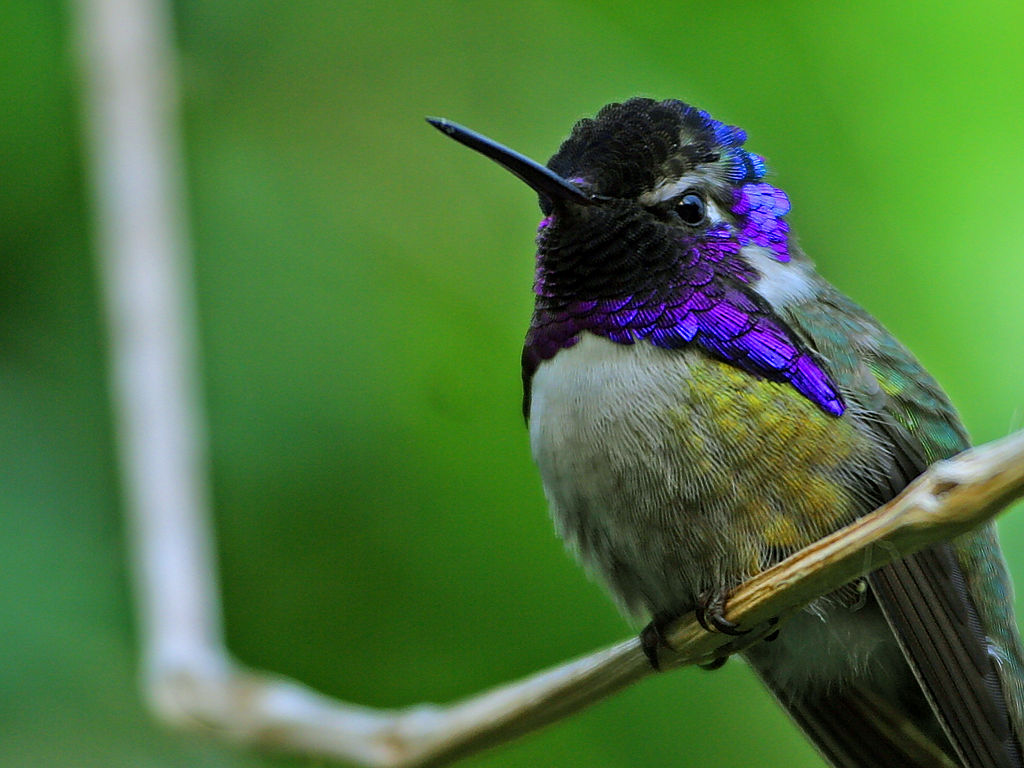
\includegraphics[width=0.8\textwidth]{figures/Hummingbird.jpg}
 	\caption{Eine Veilchenkopfelfe (auch Costakolibri genannt, vom lateinischen Calypte costae), die zur Familie der Kolibris geh\"{o}rt \cite{Kolibri}}
 	\label{fig:kolibri}
 \end{figure}
 
 \section{Erste Zwischen\"{u}berschrift}
 \label{sec:ErsteZwischenueberschrift}
 Die Arbeit kann auch Tabellen im \texttt{table}-Environment enthalten:
 \begin{table}[ht]
 	\centering
 	\caption{Entfernungstabelle S\"{u}ddeutschland, vgl. \cite{entfernungstabelle}}
 	\begin{tabular}{c r r r}
 		\toprule
 		& Augsburg & M\"{u}nchen & Stuttgart \\
 		\midrule
 		Augsburg  & -        & 61      & 149       \\
 		M\"{u}nchen   & 61       & -       & 210       \\
 		Stuttgart & 149      & 210     & -         \\
 		\bottomrule
 	\end{tabular}
 	\label{tab:entfernungen}
 \end{table}
 
 \subsection{Erste Unter\"{u}berschrift}
 \label{sec:ErsteUnterueberschrift}
 
 Das \texttt{listings}-Paket erlaubt es, Quellcode mit Syntax-Highlighting einzubinden:
 
 \begin{lstlisting}[language=Python,float=ht,caption={Python-Programm zur Berechnung der Fakult\"{a}tsfunktion}]
 def fact(n):
 """Return the n-th factorial number"""
 if n == 0:
 return 1
 else:
 return n * fact(n-1)
 
 # Test output
 print fact(10)
 print "Done"
 \end{lstlisting}
 \label{lst:factorial}  
 
 \section{Zweite Zwischen\"{u}berschrift}
 \label{sec:ZweiteZwischenueberschrift}
 
 TEXT
 
 \chapter{Schluss}
 \label{chp:Schluss}
 
 TEXT
 
 %%% Local Variables:
 %%% mode: latex
 %%% TeX-master: "../Abschlussarbeit"
 %%% End:
 

% Anhang
%\appendix

\chapter{Beweis von P = NP}

Lorem ipsum dolor sit amet, consectetuer adipiscing elit, sed diam nonummy nibh euismod tincidunt ut laoreet dolore magna aliquam erat volutpat. Ut wisi enim ad minim veniam, quis nostrud exerci tation ullamcorper suscipit lobortis nisl ut aliquip ex ea commodo consequat.

Lorem ipsum dolor sit amet, consectetuer adipiscing elit, sed diam nonummy nibh euismod tincidunt ut laoreet dolore magna aliquam erat volutpat. Ut wisi enim ad minim veniam, quis nostrud exerci tation ullamcorper suscipit lobortis nisl ut aliquip ex ea commodo consequat.

%%% Local Variables:
%%% mode: latex
%%% TeX-master: "Report"
%%% End:


% Literaturverzeichnis
\begin{otherlanguage}{british}
	\printbibliography[heading=bibintoc]
\end{otherlanguage}

% Eidesstattliche Erklärung
\clearpage
\section*{\GetTranslation{honesty@title}}
\GetTranslation{honesty@body}

\vspace{2em}
\makeatletter
Orsay, \@date
\par\vspace{1.5cm}
(\@author)
\makeatother

%%% Local Variables:
%%% mode: latex
%%% TeX-master: "Report"
%%% End:


\end{document}

%%% Local Variables:
%%% mode: latex
%%% TeX-master: t
%%% End:
